\section{unison}
\begin{figure}[h]
\centering
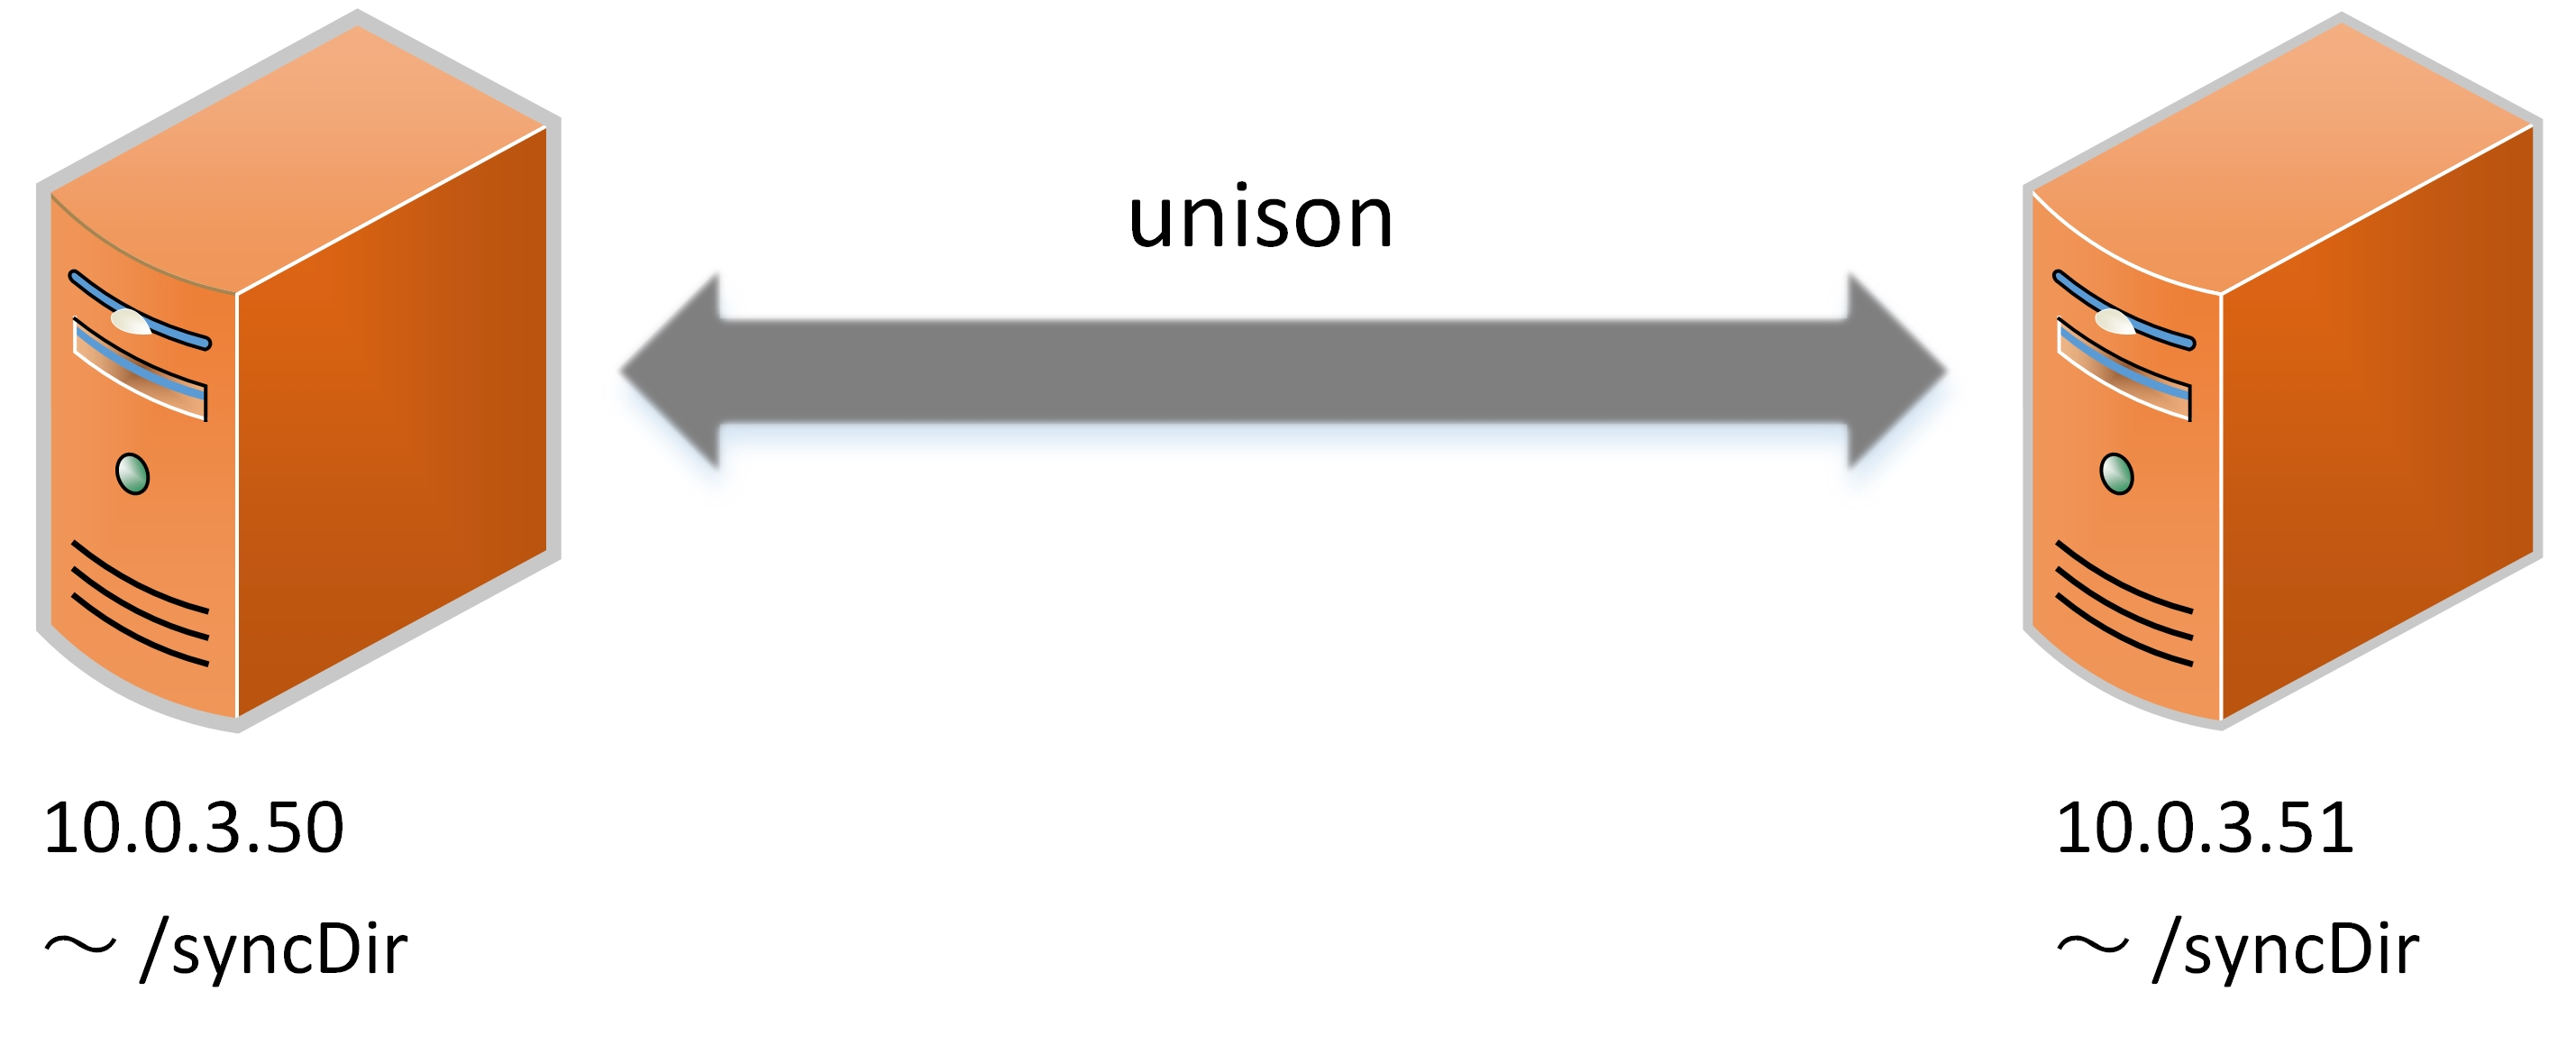
\includegraphics[width=\textwidth]{pic/unison.jpg}
\caption{unison}
\end{figure}
\subsection{安装}
两台机器上都安装如下包:\\
\shell{sudo apt-get install openssh-server inotify-tools unison -y}

\subsection{SSH互信}
两台机器上都做如下操作交换公钥:\\
\shell{ssh-keygen -t rsa -C "unisonKey"} \quad\verb"(一路回车即可)"\\
\shell{ssh-copy-id -i .ssh/id\_rsa.pub ubuntu@10.0.3.50} \quad\verb"(另一台机器)"\\ 
\shell{ssh-copy-id -i .ssh/id\_rsa.pub ubuntu@10.0.3.51}
\par
当然也可以将生成的公钥手动复制到 $\sim$/.ssh/authorized\_keys 文件中,每个公钥单独一行.

\subsection{配置}
设置unison默认的配置文件并添加内容:\\
\shell{vim $\sim$/.unison/default.prf}
\begin{verbatim}
#接受默认动作并执行,遇到冲突文件自动跳过
batch = true
#表示保持同步的文件属主信息。
owner = true
#表示保持同步的文件属组信息。
group = true
#表示保持同步的文件读写权限。
perms = -1
#快速检测,使用文件的修改时间和文件长度来比较两地文件
fastcheck = true
#默认值为true,表示当需要同步的两个目录有一个为空时,unison将停止。
confirmbigdel = false
#默认值是true,用于激活rsync传输模式。
rsync = false
#使用ssh的压缩传输方式。
sshargs = -C
#优化传输参数,默认值为true。
xferbycopying = true
#除了错误信息,不打印任何信息
silent = true
#指定日志文件
logfile = /home/ubuntu/.unison/AB.log
\end{verbatim}

配置文件直接发送到另一台机器即可:\\
\shell{scp $\sim$/.unison/default.prf ubuntu@10.0.3.51:$\sim$/.unison/default.prf} 

\subsection{使用inotify}
编写如下脚本:\\
\shell{vim $\sim$/unison.sh}
\begin{verbatim}
#!/bin/bash
remotehost=10.0.3.51    
src=/home/ubuntu/syncDir/
/usr/bin/inotifywait -mrq --timefmt '%d/%m/%y %H:%M' --format \
'%T %w%f%e' -e close_write,modify,delete,create,attrib,move $src \
| while read files
    do
    /usr/bin/unison $src ssh://ubuntu@$remotehost/$src
    done
\end{verbatim}

复制到另一台机器并修改一行:\\
\shell{scp $\sim$/unison.sh ubuntu@10.0.3.51:$\sim$/unison.sh} \\
\texttt{remotehost=10.0.3.50}

\par
两台机器都做如下操作:\\
\shell{mkdir $\sim$/syncDir}\\
\shell{chmod +x $\sim$/unison.sh}\\
\shell{$\sim$/unison.sh \&}

\par
接下来即可测试同步效果了. 关于inotifywait的更多信息和unison更多配置参数见“有道笔记”. 